En este capítulo se detalla la metodología y los resultados del proceso de validación del prototipo de \textit{Reset}. Para evaluar la viabilidad de la propuesta híbrida, la calidad de los controles, la curva de dificultad y la coherencia del diseño general, se sometió el videojuego a una sesión de pruebas con usuarios finales seguida de un cuestionario cuantitativo y cualitativo.

% =========================================================================
\section{Metodología y Perfil de los Evaluadores}
La muestra de evaluación estuvo compuesta por un grupo de $10$ usuarios que testearon la versión final del prototipo completo. Tras la sesión de juego, los usuarios completaron un cuestionario estructurado en tres bloques principales: perfil demográfico, hábitos como jugador y experiencia detallada con \textit{Reset}.

\subsection{Bloque Demográfico}
El análisis de la muestra arroja un perfil homogéneo de evaluadores:
\begin{itemize}
    \item \textbf{Edad:} El $100\%$ de los evaluadores se sitúa en el rango de edad de entre $20$ y $25$ años, tal y como se detalla en los resultados de la Figura~\ref{fig:val:edad}.
    \begin{figure}[H]
        \centering
        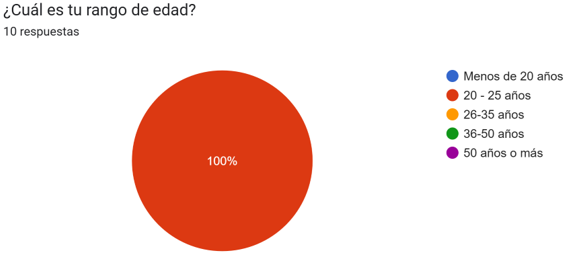
\includegraphics[width=0.85\textwidth]{pages/img/Edad.png}
        \caption{Resultados del cuestionario: Rango de edad de los evaluadores.}
        \label{fig:val:edad}
    \end{figure}
    
    \item \textbf{Género:} La totalidad de la muestra de evaluación ($100\%$) es de género masculino, según se representa en la Figura~\ref{fig:val:sexo}.
    \begin{figure}[H]
        \centering
        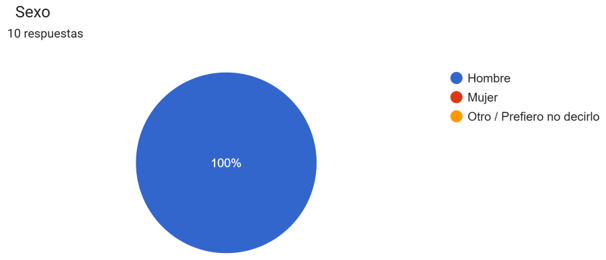
\includegraphics[width=0.85\textwidth]{pages/img/Sexo.png}
        \caption{Resultados del cuestionario: Género de los evaluadores.}
        \label{fig:val:sexo}
    \end{figure}
    
    \item \textbf{Ámbito Profesional/Académico:} El $70\%$ de los usuarios pertenece al sector de la Informática y la Ingeniería, mientras que un $20\%$ son estudiantes de otros ámbitos y un $10\%$ pertenece a otros sectores laborales, tal como ilustra la Figura~\ref{fig:val:conocimiento}. Este perfil de evaluadores con trasfondo técnico proporciona un valor añadido, ya que sus comentarios cualitativos tienen una base analítica sobre el rendimiento del software.
    \begin{figure}[H]
        \centering
        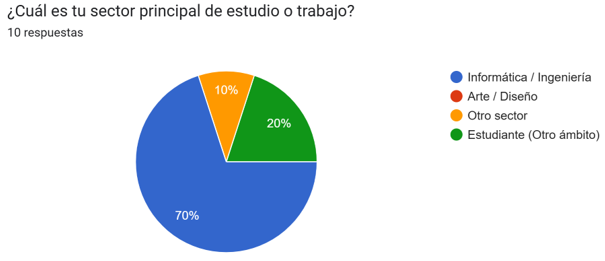
\includegraphics[width=0.85\textwidth]{pages/img/Conocimiento.png}
        \caption{Resultados del cuestionario: Sector de estudio o trabajo de los evaluadores.}
        \label{fig:val:conocimiento}
    \end{figure}
\end{itemize}

\subsection{Perfil de Jugador}
Los hábitos de consumo de videojuegos de los evaluadores indican que nos encontramos ante un grupo de jugadores con perfiles diversos:
\begin{itemize}
    \item \textbf{Frecuencia de Juego:} El $40\%$ juega a diario y el $30\%$ lo hace varias veces a la semana. Un $20\%$ juega ocasionalmente y solo el $10\%$ casi nunca (ver Figura~\ref{fig:val:frecuencia}).
    \begin{figure}[H]
        \centering
        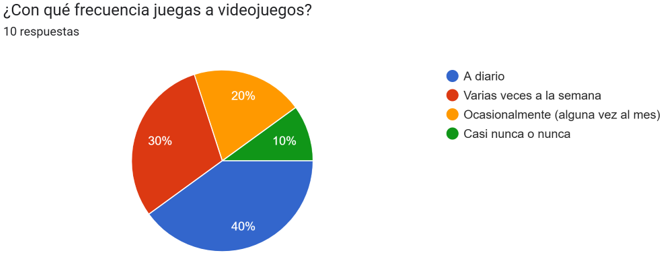
\includegraphics[width=0.85\textwidth]{pages/img/Frecuencia.png}
        \caption{Resultados del cuestionario: Frecuencia de juego semanal.}
        \label{fig:val:frecuencia}
    \end{figure}
    
    \item \textbf{Plataformas Habituales:} El $70\%$ consume juegos en dispositivos móviles, mientras que el $60\%$ utiliza el PC y otro $60\%$ consolas de sobremesa (opción de respuesta múltiple, ver Figura~\ref{fig:val:plataformas}).
    \begin{figure}[H]
        \centering
        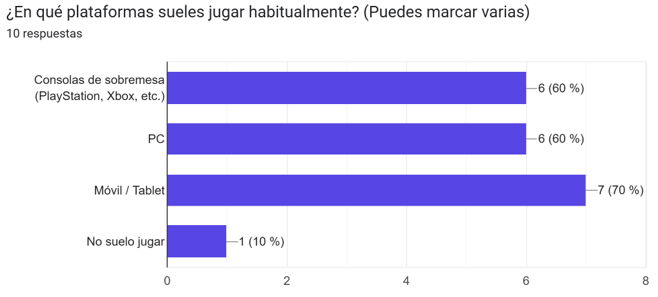
\includegraphics[width=0.85\textwidth]{pages/img/Plataformas.png}
        \caption{Resultados del cuestionario: Plataformas de juego habituales.}
        \label{fig:val:plataformas}
    \end{figure}
    
    \item \textbf{Géneros Preferidos:} El género de Acción y Supervivencia es el preferido por el $70\%$ de los usuarios, seguido por los deportes ($40\%$), \textit{shooters} ($30\%$) y las plataformas ($20\%$). Esta distribución (mostrada en la Figura~\ref{fig:val:generos}) aporta un gran valor para comparar la jugabilidad entre los dos mundos del juego, permitiendo contextualizar las valoraciones físicas con base en la experiencia previa de los usuarios en géneros dispares.
    \begin{figure}[H]
        \centering
        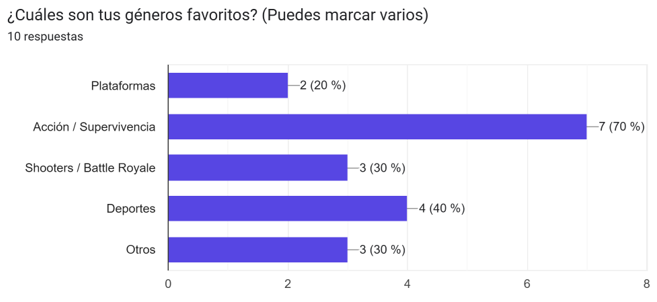
\includegraphics[width=0.85\textwidth]{pages/img/Generos.png}
        \caption{Resultados del cuestionario: Géneros preferidos.}
        \label{fig:val:generos}
    \end{figure}
    
    \item \textbf{Zona de Confort y Apertura Narrativa:} El $60\%$ de los jugadores admite que tiende a repetir géneros dentro de su zona de confort (representado en la Figura~\ref{fig:val:estancamiento}), mientras que el $40\%$ restante manifiesta una búsqueda activa de experiencias jugables variadas.
    \begin{figure}[H]
        \centering
        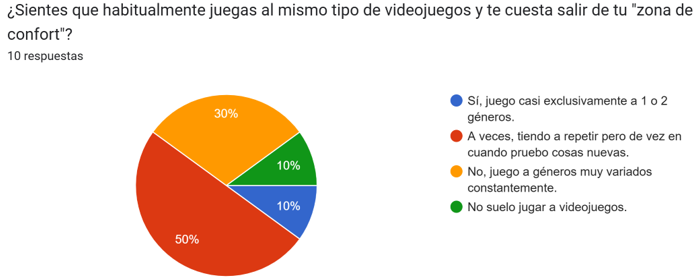
\includegraphics[width=0.85\textwidth]{pages/img/Estancamiento.png}
        \caption{Resultados del cuestionario: Zona de confort en géneros de juego.}
        \label{fig:val:estancamiento}
    \end{figure}
    
    \item \textbf{Flexibilidad por Narrativa:} El $90\%$ de los usuarios valida en algún grado la importancia de la narrativa como factor condicionante para experimentar mecánicas o géneros inusuales. Esto confirma que el hilo conductor narrativo resulta crítico para la aceptación de la propuesta, como detalla la Figura~\ref{fig:val:enganche}.
    \begin{figure}[H]
        \centering
        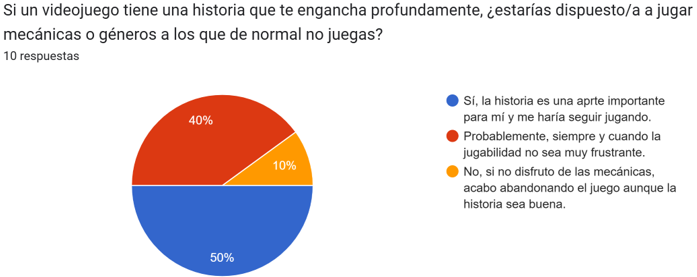
\includegraphics[width=0.85\textwidth]{pages/img/Enganche.png}
        \caption{Resultados del cuestionario: Flexibilidad y enganche por narrativa.}
        \label{fig:val:enganche}
    \end{figure}
    
    \item \textbf{Barreras de Abandono:} La falta de tiempo es la principal causa de abandono de un juego para el $80\%$ de la muestra, seguida de los controles confusos o frustrantes ($40\%$) y mecánicas repetitivas ($30\%$), según los resultados de la Figura~\ref{fig:val:abandono}.
    \begin{figure}[H]
        \centering
        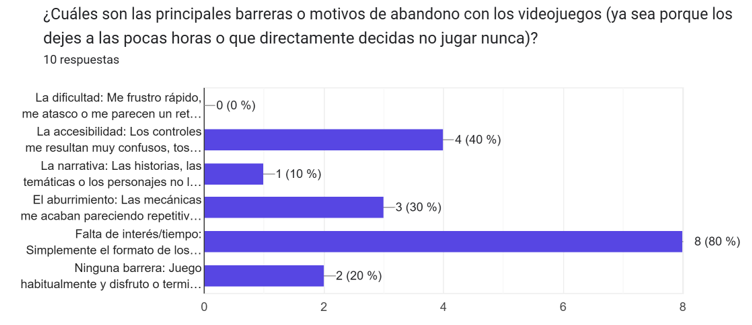
\includegraphics[width=0.85\textwidth]{pages/img/Abandono.png}
        \caption{Resultados del cuestionario: Barreras o motivos de abandono.}
        \label{fig:val:abandono}
    \end{figure}
\end{itemize}

% =========================================================================
\section{Análisis Cuantitativo de la Experiencia con \textit{Reset}}
El bloque principal del cuestionario evaluó la percepción de los usuarios sobre el rendimiento, la jugabilidad y la estética de \textit{Reset} empleando preguntas de opción cerrada y escalas del 1 (valoración más baja) al 5 (valoración más alta).

\subsection{Fluidez, Controles y Rendimiento}
La experiencia técnica general del prototipo ha sido calificada como notablemente estable:
\begin{itemize}
    \item El $50\%$ de los usuarios declaró haber tenido una experiencia de juego completamente fluida. El $40\%$ detectó pequeños errores leves que no afectaron a la jugabilidad, y solo un $10\%$ experimentó algún fallo relevante asociado a las rutinas físicas o lógicas de transición (ver la gráfica de la Figura~\ref{fig:val:fluidez}).
    \begin{figure}[H]
        \centering
        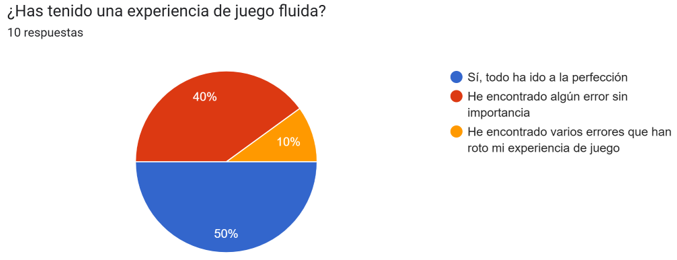
\includegraphics[width=0.85\textwidth]{pages/img/Fluidez.png}
        \caption{Resultados del cuestionario: Fluidez técnica de la experiencia.}
        \label{fig:val:fluidez}
    \end{figure}
    
    \item La respuesta física y fluidez de los controles obtuvo una valoración excelente: el $30\%$ la calificó con la puntuación máxima ($5/5$) y el $60\%$ con un $4/5$, mientras que solo un $10\%$ le otorgó una valoración intermedia o neutral ($3/5$), como refleja la Figura~\ref{fig:val:controles}.
    \begin{figure}[H]
        \centering
        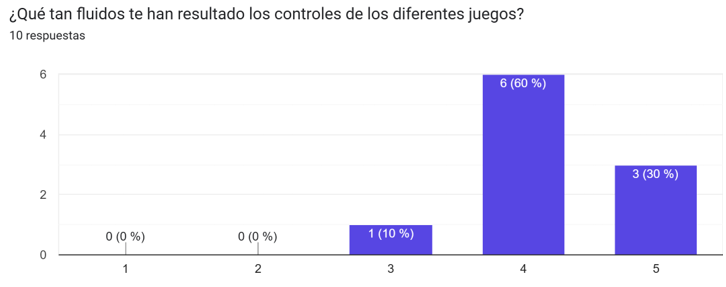
\includegraphics[width=0.85\textwidth]{pages/img/Controles.png}
        \caption{Resultados del cuestionario: Valoración del control del personaje.}
        \label{fig:val:controles}
    \end{figure}
\end{itemize}

\subsection{Curva de Dificultad y Balanceo de Sistemas}
La valoración sobre la dificultad del juego se concentró mayoritariamente en el valor central:
\begin{itemize}
    \item El $70\%$ de los usuarios otorgó una puntuación de $3/5$ (dificultad equilibrada), mientras que un $20\%$ la consideró fácil ($2/5$) y un $10\%$ difícil ($4/5$), como se observa en la Figura~\ref{fig:val:dificultad}.
    \begin{figure}[H]
        \centering
        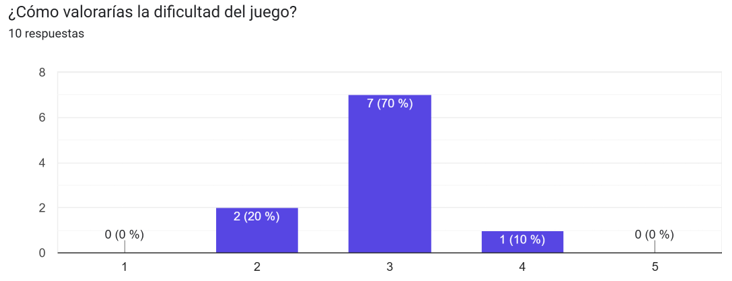
\includegraphics[width=0.85\textwidth]{pages/img/Dificultad.png}
        \caption{Resultados del cuestionario: Valoración de la dificultad general.}
        \label{fig:val:dificultad}
    \end{figure}
    
    \item El comportamiento de la Inteligencia Artificial y el diseño de los puzles cenitales fueron evaluados con un $40\%$ de notas notables ($4/5$) y un $30\%$ de excelentes ($5/5$), mientras que el $30\%$ restante asignó una valoración neutral ($3/5$), según ilustra la Figura~\ref{fig:val:iapuzle}.
    \begin{figure}[H]
        \centering
        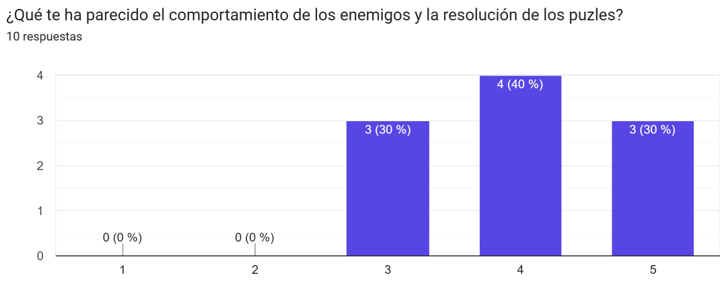
\includegraphics[width=0.85\textwidth]{pages/img/IAPuzle.png}
        \caption{Resultados del cuestionario: Comportamiento de IA y puzles.}
        \label{fig:val:iapuzle}
    \end{figure}
    
    \item Las mecánicas y acciones del personaje fueron consideradas completas y suficientes para la resolución de los niveles por el $80\%$ de los jugadores (calificaciones de 4 y 5), dejando solo un $20\%$ en una percepción de suficiencia límite ($3/5$), tal como muestra la Figura~\ref{fig:val:mecanicas}.
    \begin{figure}[H]
        \centering
        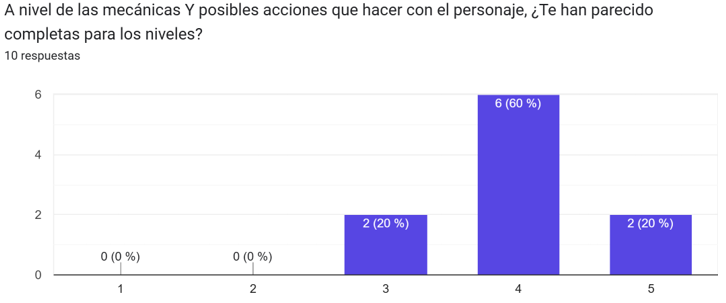
\includegraphics[width=0.85\textwidth]{pages/img/Mecanicas.png}
        \caption{Resultados del cuestionario: Completitud de las mecánicas.}
        \label{fig:val:mecanicas}
    \end{figure}
\end{itemize}

\subsection{Estética, Coherencia e Inmersión de la Hibridación}
Uno de los mayores temores de diseño al combinar una perspectiva cenital en el Mundo 1 con un plataformas lateral en el Mundo 2 era la pérdida de inmersión del jugador. Los resultados cuantitativos han respaldado con éxito la resolución de este apartado:
\begin{itemize}
    \item El $100\%$ de los encuestados consideró que el diseño visual, la ambientación y la estética de cada zona son plenamente coherentes con la narrativa, reflejado en la Figura~\ref{fig:val:estetica}.
    \begin{figure}[H]
        \centering
        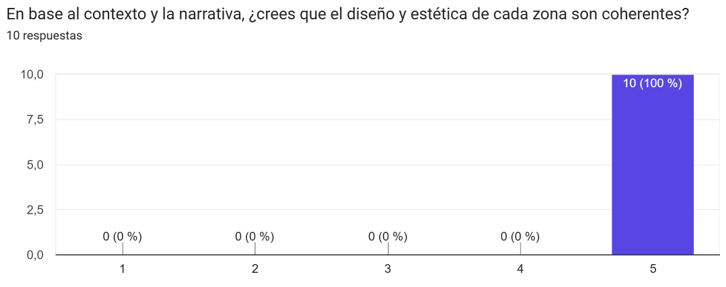
\includegraphics[width=0.85\textwidth]{pages/img/Estetica.png}
        \caption{Resultados del cuestionario: Coherencia estética entre niveles.}
        \label{fig:val:estetica}
    \end{figure}
    
    \item En cuanto a la valoración sobre la intuitividad de la interfaz (UI) y la navegación por los menús del juego, el $60\%$ otorgó la nota máxima ($5/5$), el $30\%$ un $4/5$ y el $10\%$ restante un $3/5$, lo que representa una aceptación notable con margen de optimización en futuras revisiones, detallado en la Figura~\ref{fig:val:interfaz}.
    \begin{figure}[H]
        \centering
        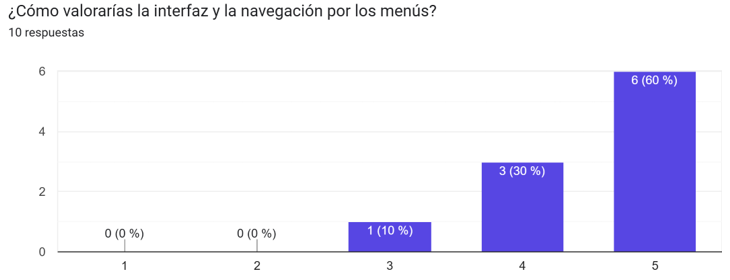
\includegraphics[width=0.85\textwidth]{pages/img/UIUX.png}
        \caption{Resultados del cuestionario: Valoración de la interfaz y menús.}
        \label{fig:val:interfaz}
    \end{figure}
    
    \item En base al grado de satisfacción general tras haber jugado al prototipo, el $70\%$ de los usuarios mostró un interés máximo ($5/5$) y el $30\%$ un interés alto ($4/5$) en seguir participando en el desarrollo futuro de \textit{Reset}, evidenciando un elevado nivel de fidelización y aceptación de la experiencia jugable, tal como ilustra la Figura~\ref{fig:val:satisfaccion}.
    \begin{figure}[H]
        \centering
        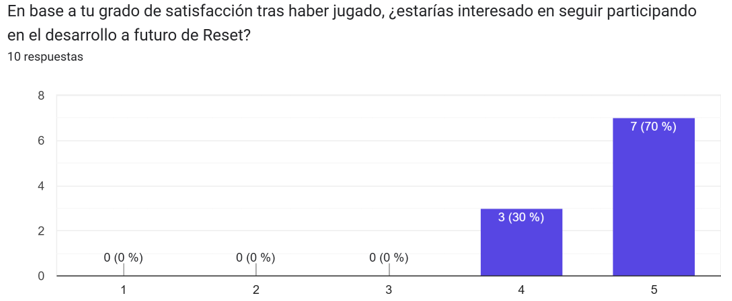
\includegraphics[width=0.85\textwidth]{pages/img/Satisfaccion.png}
        \caption{Resultados del cuestionario: Interés en el desarrollo futuro.}
        \label{fig:val:satisfaccion}
    \end{figure}
    
    \item Probar este prototipo despertó el interés de los usuarios por jugar a otros géneros fuera de su zona de confort, obteniendo un $40\%$ de votos máximos ($5/5$) y un $50\%$ de votos notables ($4/5$), mientras que el $10\%$ restante mostró una postura neutral, correspondiente a perfiles de juego más especializados (ver la Figura~\ref{fig:val:disfrute}).
    \begin{figure}[H]
        \centering
        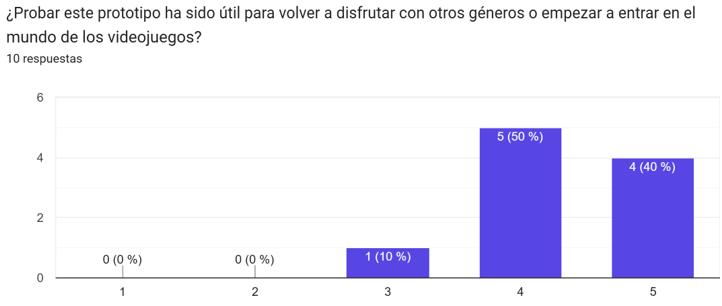
\includegraphics[width=0.85\textwidth]{pages/img/Disfrute.png}
        \caption{Resultados del cuestionario: Interés en descubrir otros géneros.}
        \label{fig:val:disfrute}
    \end{figure}
    
    \item Ante la pregunta de si el cambio de estética y de género afectaba a su inmersión en la partida, el $80\%$ afirmó que no afectó en absoluto y que se mantuvo inmerso en todo momento, mientras que el $20\%$ restante manifestó un impacto inicial moderado pero mantuvo la inmersión general durante el transcurso de la partida (ver la Figura~\ref{fig:val:inmersion}).
    \begin{figure}[H]
        \centering
        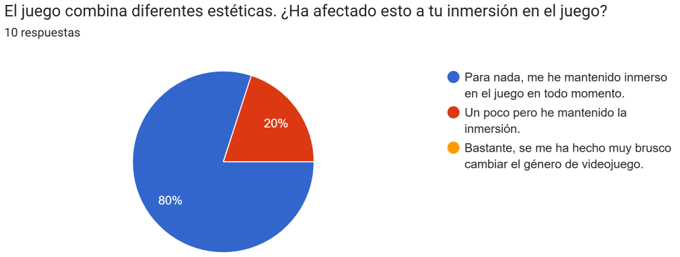
\includegraphics[width=0.85\textwidth]{pages/img/Inmersion.png}
        \caption{Resultados del cuestionario: Impacto de la mezcla de estéticas en la inmersión.}
        \label{fig:val:inmersion}
    \end{figure}
\end{itemize}

% =========================================================================
\section{Análisis Cualitativo y Áreas de Mejora}
Las preguntas abiertas permitieron recolectar opiniones detalladas sobre las fortalezas del juego y las áreas que requieren iteración o corrección antes de un lanzamiento comercial. La totalidad de las respuestas cualitativas y opiniones literales aportadas por los evaluadores se encuentran recopiladas de forma estructurada en el Apéndice~\ref{sec:apendice_comentarios} de esta memoria.

\subsection{Fortalezas del Videojuego}
Los usuarios coincidieron en destacar cuatro aspectos altamente positivos de la obra:
\begin{enumerate}
    \item \textbf{La Coherencia en la Hibridación:} Se alabó de manera unánime la transición estética y de control entre mundos, logrando que dos géneros tan dispares se sientan parte del mismo hilo conductor narrativo.
    \item \textbf{La Fluidez del Control de Plataformas:} Los jugadores destacaron la responsividad del avatar en el Mundo 2 (\textit{Super Reset Bros}), especialmente al realizar mecánicas avanzadas como el encadenamiento de rebotes sobre cabezas de enemigos y los saltos con \textit{dash} y deslizamiento por paredes.
    \item \textbf{La Ambientación y el Pulido de la UI:} Se valoró muy positivamente el diseño visual pixel art, la música y el acabado de las interfaces del menú principal y de pausa.
    \item \textbf{Aspectos Narrativos y Referencias:} Los evaluadores destacaron de forma muy positiva la inclusión de referencias culturales a títulos clásicos de la industria, así como la estructuración lógica y el diseño de los puzles integrados en la historia.
\end{enumerate}

\subsection{Áreas de Mejora e Incidencias Detectadas}
El análisis cualitativo reveló los siguientes aspectos de diseño y programación que deben ser revisados:
\begin{itemize}
    \item \textbf{Pico de Dificultad Excesivo en Mundo 2 (Nivel 2):} Varios usuarios no familiarizados con los juegos de plataformas hardcore reportaron que la primera mitad del Nivel 2 es asequible, pero la sección de plataformas móviles y bloques inestables combinados con zonas estrechas de pinchos presenta una curva de dificultad demasiado empinada. Esto provocó la frustración de algunos evaluadores que no pudieron completar el nivel.
    \item \textbf{Densidad de Enemigos en Mundo 1 (Nivel 1):} Se sugirió reducir el número de infectados iniciales en el Nivel 1 para permitir una introducción más suave a las mecánicas de disparo y sigilo.
    \item \textbf{Bug en el Sistema de Persistencia y Carga:} Un usuario reportó un bug crítico donde, al guardar la partida en el Nivel 2 del Mundo 2, el gestor reinició su posición al Nivel 1, impidiendo el progreso normal. Esto apunta a una inconsistencia de lectura en el método \texttt{LoadGame()} del \texttt{SaveManager}.
    \item \textbf{Mapeado de Controles Estático:} Se recomendó añadir una opción de reconfiguración de teclas (*Key Binding*) en caliente para facilitar la transición de control entre la perspectiva cenital y el avance lateral.
\end{itemize}

% =========================================================================
\section{Conclusiones de la Validación}
El proceso de evaluación valida de forma muy positiva los pilares conceptuales del proyecto. En primer lugar, se ha resuelto con éxito la conectividad narrativa entre mundos de géneros dispares, un aspecto que inicialmente representaba un reto de diseño crítico. La integración de puzles y referencias culturales no solo consolidó la inmersión de los jugadores habituales, sino que también facilitó el acceso a perfiles menos experimentados gracias al hilo conductor de la historia.

En segundo lugar, se destaca el rendimiento y el pulido del apartado mecánico, especialmente en el Mundo 2 (\textit{Super Reset Bros}). Los evaluadores señalaron la fluidez y responsividad del personaje al encadenar acciones aéreas y rebotes, lo que corrobora la efectividad del refinamiento de las físicas de movimiento y el comportamiento de los enemigos.

Finalmente, como línea de mejora fundamental, la validación expone la necesidad de reajustar tanto la curva de dificultad del Mundo 2 como los posibles errores puntuales que hayan sufrido los usuarios. Aunque el diseño pretendía ofrecer una experiencia híbrida y retadora para jugadores avanzados a la vez que asequible para noveles, el resultado final presenta un pico de dificultad excesivo en el segundo nivel. La disposición de los usuarios a continuar colaborando en futuras iteraciones del proyecto confirma el interés que suscita \textit{Reset} y proporciona una base sólida para implementar estos ajustes mecánicos antes de una versión definitiva.